% periodic-shear-layer.tex

\section{Periodic Shear Layer}\index{boundary conditions!periodic!example of use}
\label{periodic-shear-layer-sec}
%
This example shows the use of the Python functions to set up
a simple shear flow with a linear variation of velocity through the finite-width shear layer.
There is also a variation of species mass fractions of helium and air between the counterflowing streams.
The basic flow is intended to be somewhat representative of the fuel-air mixing layers
encountered in shock-tunnel tests of scramjets, however, the model flow here
is made periodic in the $x$-direction by connecting the block faces as shown in
Fig.\,\ref{psl-layout-fig}. 

\begin{figure}[htbp]
\begin{center}
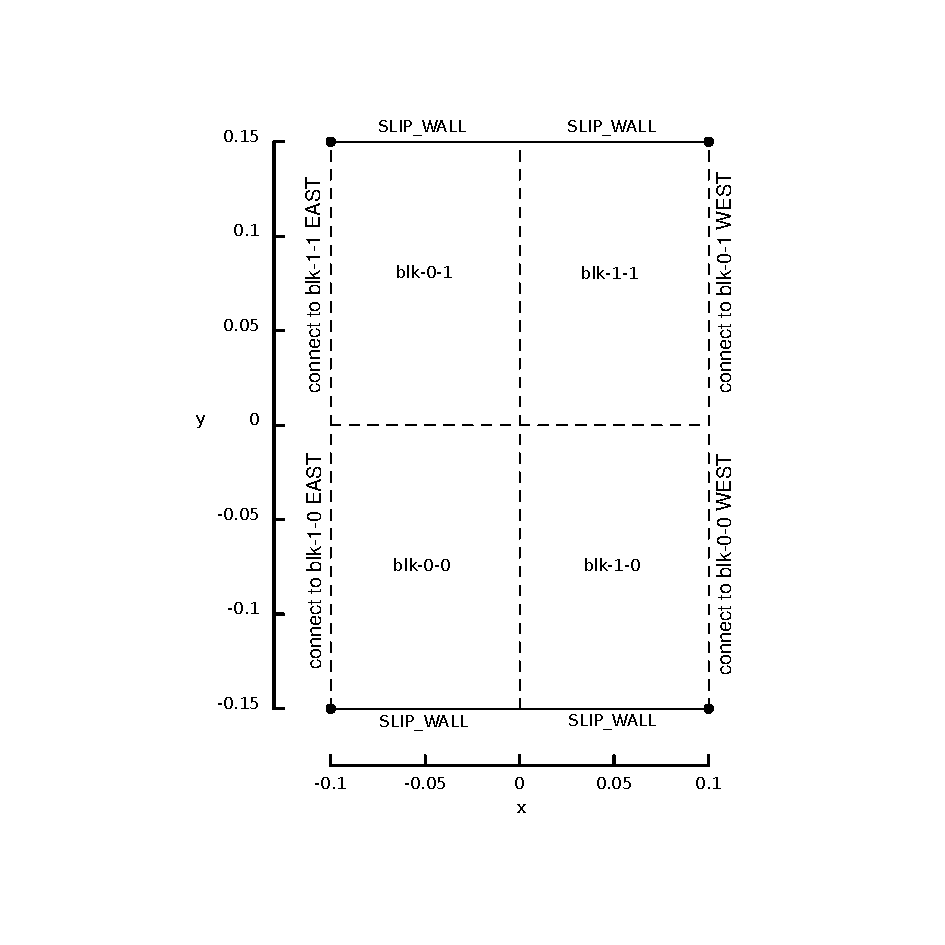
\includegraphics[width=10cm,viewport=94 63 353 396,clip=true]{../2D/periodic-shear-layer/psl-layout.pdf}
\end{center}
\caption{Computational domain for the periodic shear layer.}
\label{psl-layout-fig}
\end{figure}

\medskip
Figure\,\ref{psl-mass-fraction-fig} shows the mass fraction of helium at several time instants through
the evolution of the shear layer.
The layer has started with almost parallel flow, with a relatively small velocity perturbation,
as defined in the function \texttt{initial\_gas()} in the input script (see Sec.\,\ref{psl-py-file}).

\clearpage

\begin{figure}[htbp]
\begin{center}
\mbox{
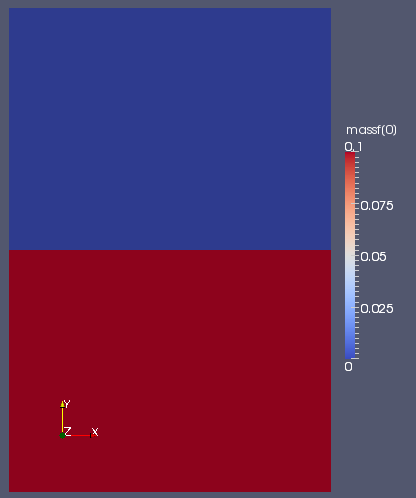
\includegraphics[width=0.25\textwidth]{../2D/periodic-shear-layer/psl-massf0-t00.png}
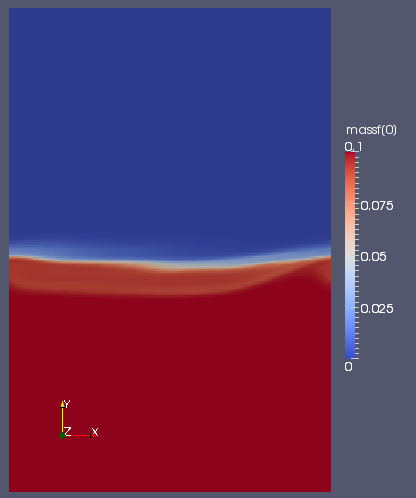
\includegraphics[width=0.25\textwidth]{../2D/periodic-shear-layer/psl-massf0-t05.png}
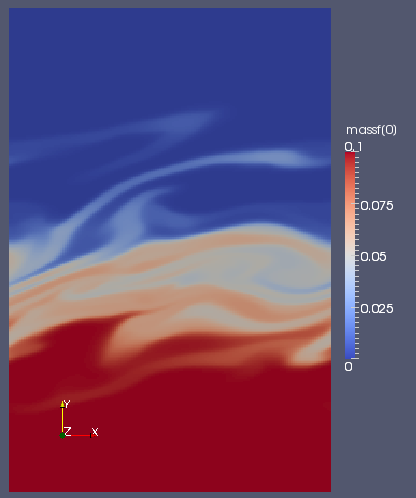
\includegraphics[width=0.25\textwidth]{../2D/periodic-shear-layer/psl-massf0-t10.png}
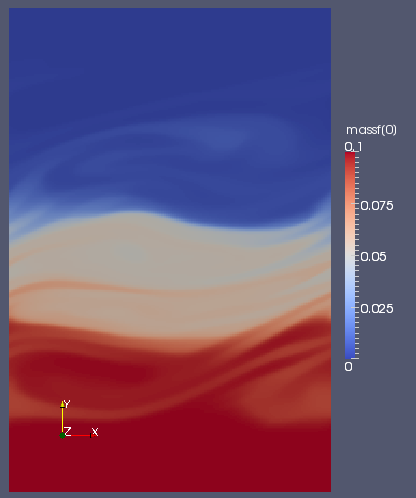
\includegraphics[width=0.25\textwidth]{../2D/periodic-shear-layer/psl-massf0-t15.png}
}
\end{center}
\caption{Mass fraction for helium across the periodic shear layer at times 0, 5.1\,ms, 10.2\,ms and 15\,ms.}
\label{psl-mass-fraction-fig}
\end{figure}

\medskip
Figure\,\ref{psl-vorticity-fig} shows the evolution of the vorticity field.
Vorticity is not part of the flow data files but can be computed within \texttt{Paraview}
by applying the following filters to the cell data:
\begin{itemize}
 \item \texttt{Gradient of Unstructured DataSet} selecting \texttt{vel.x} as the scalar and
    \texttt{du} as the result array name.
 \item \texttt{Gradient of Unstructured DataSet} selecting \texttt{vel.y} as the scalar and
    \texttt{dv} as the result array name.
 \item \texttt{Calculator} with \texttt{Cell Data} as the attribute mode, 
    \texttt{dv\_X - du\_Y} as the expression to compute, and \texttt{vorticity} as the result array name.
\end{itemize}
Note that there is a small defect in the vorticity values at the block boundaries.
This is an artifact of the \texttt{Paraview} calculation and not of the original simulation flow field.
 
\begin{figure}[htbp]
\begin{center}
\mbox{
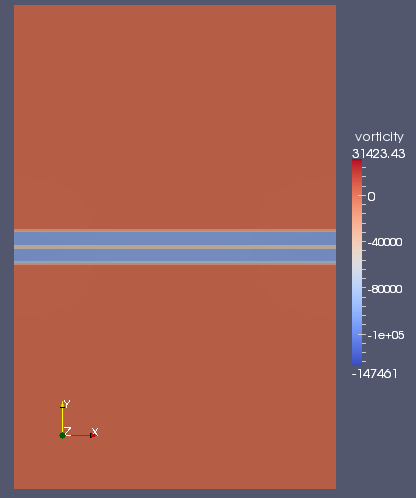
\includegraphics[width=0.25\textwidth]{../2D/periodic-shear-layer/psl-vorticity-t00.png}
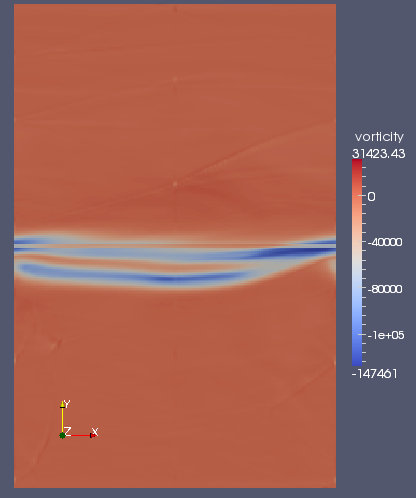
\includegraphics[width=0.25\textwidth]{../2D/periodic-shear-layer/psl-vorticity-t05.png}
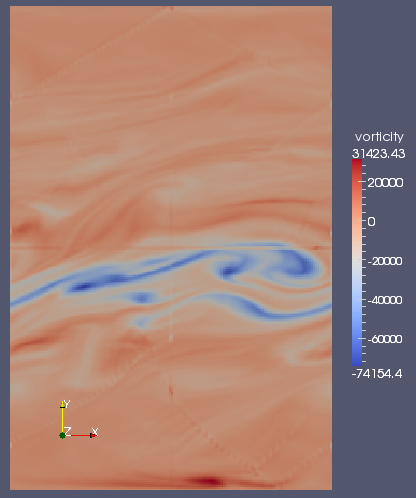
\includegraphics[width=0.25\textwidth]{../2D/periodic-shear-layer/psl-vorticity-t10.png}
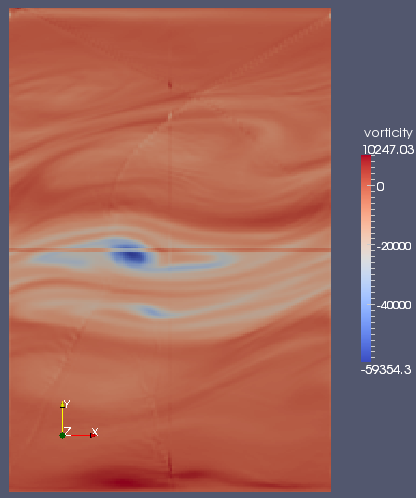
\includegraphics[width=0.25\textwidth]{../2D/periodic-shear-layer/psl-vorticity-t15.png}
}
\end{center}
\caption{Vorticity field for the periodic shear layer at times 0, 5.1\,ms, 10.2\,ms and 15\,ms.}
\label{psl-vorticity-fig}
\end{figure}

\newpage

\subsection{Input script (.py)}
\label{psl-py-file}
\index{FlowCondition!add\_to\_list parameter!example of use}
\topbar
\lstinputlisting[language={}]{../2D/periodic-shear-layer/psl.py}
\bottombar


\subsection{Shell scripts}
\label{psl-sh-files}
\topbar
\lstinputlisting[language={}]{../2D/periodic-shear-layer/prep_simulation.sh}
\bottombar \\
\topbar
\lstinputlisting[language={}]{../2D/periodic-shear-layer/run_simulation.sh}
\bottombar

\subsection{Notes}
\begin{itemize}
\item This simulation take 33707 steps and 28945\,seconds on 4 cores of geyser (AMD processors).
\end{itemize}
